% Options for packages loaded elsewhere
\PassOptionsToPackage{unicode}{hyperref}
\PassOptionsToPackage{hyphens}{url}
\PassOptionsToPackage{dvipsnames,svgnames,x11names}{xcolor}
%
\documentclass[
  letterpaper,
  DIV=11,
  numbers=noendperiod]{scrartcl}

\usepackage{amsmath,amssymb}
\usepackage{iftex}
\ifPDFTeX
  \usepackage[T1]{fontenc}
  \usepackage[utf8]{inputenc}
  \usepackage{textcomp} % provide euro and other symbols
\else % if luatex or xetex
  \usepackage{unicode-math}
  \defaultfontfeatures{Scale=MatchLowercase}
  \defaultfontfeatures[\rmfamily]{Ligatures=TeX,Scale=1}
\fi
\usepackage{lmodern}
\ifPDFTeX\else  
    % xetex/luatex font selection
\fi
% Use upquote if available, for straight quotes in verbatim environments
\IfFileExists{upquote.sty}{\usepackage{upquote}}{}
\IfFileExists{microtype.sty}{% use microtype if available
  \usepackage[]{microtype}
  \UseMicrotypeSet[protrusion]{basicmath} % disable protrusion for tt fonts
}{}
\makeatletter
\@ifundefined{KOMAClassName}{% if non-KOMA class
  \IfFileExists{parskip.sty}{%
    \usepackage{parskip}
  }{% else
    \setlength{\parindent}{0pt}
    \setlength{\parskip}{6pt plus 2pt minus 1pt}}
}{% if KOMA class
  \KOMAoptions{parskip=half}}
\makeatother
\usepackage{xcolor}
\setlength{\emergencystretch}{3em} % prevent overfull lines
\setcounter{secnumdepth}{5}
% Make \paragraph and \subparagraph free-standing
\ifx\paragraph\undefined\else
  \let\oldparagraph\paragraph
  \renewcommand{\paragraph}[1]{\oldparagraph{#1}\mbox{}}
\fi
\ifx\subparagraph\undefined\else
  \let\oldsubparagraph\subparagraph
  \renewcommand{\subparagraph}[1]{\oldsubparagraph{#1}\mbox{}}
\fi


\providecommand{\tightlist}{%
  \setlength{\itemsep}{0pt}\setlength{\parskip}{0pt}}\usepackage{longtable,booktabs,array}
\usepackage{calc} % for calculating minipage widths
% Correct order of tables after \paragraph or \subparagraph
\usepackage{etoolbox}
\makeatletter
\patchcmd\longtable{\par}{\if@noskipsec\mbox{}\fi\par}{}{}
\makeatother
% Allow footnotes in longtable head/foot
\IfFileExists{footnotehyper.sty}{\usepackage{footnotehyper}}{\usepackage{footnote}}
\makesavenoteenv{longtable}
\usepackage{graphicx}
\makeatletter
\def\maxwidth{\ifdim\Gin@nat@width>\linewidth\linewidth\else\Gin@nat@width\fi}
\def\maxheight{\ifdim\Gin@nat@height>\textheight\textheight\else\Gin@nat@height\fi}
\makeatother
% Scale images if necessary, so that they will not overflow the page
% margins by default, and it is still possible to overwrite the defaults
% using explicit options in \includegraphics[width, height, ...]{}
\setkeys{Gin}{width=\maxwidth,height=\maxheight,keepaspectratio}
% Set default figure placement to htbp
\makeatletter
\def\fps@figure{htbp}
\makeatother
\newlength{\cslhangindent}
\setlength{\cslhangindent}{1.5em}
\newlength{\csllabelwidth}
\setlength{\csllabelwidth}{3em}
\newlength{\cslentryspacingunit} % times entry-spacing
\setlength{\cslentryspacingunit}{\parskip}
\newenvironment{CSLReferences}[2] % #1 hanging-ident, #2 entry spacing
 {% don't indent paragraphs
  \setlength{\parindent}{0pt}
  % turn on hanging indent if param 1 is 1
  \ifodd #1
  \let\oldpar\par
  \def\par{\hangindent=\cslhangindent\oldpar}
  \fi
  % set entry spacing
  \setlength{\parskip}{#2\cslentryspacingunit}
 }%
 {}
\usepackage{calc}
\newcommand{\CSLBlock}[1]{#1\hfill\break}
\newcommand{\CSLLeftMargin}[1]{\parbox[t]{\csllabelwidth}{#1}}
\newcommand{\CSLRightInline}[1]{\parbox[t]{\linewidth - \csllabelwidth}{#1}\break}
\newcommand{\CSLIndent}[1]{\hspace{\cslhangindent}#1}

\usepackage{booktabs}
\usepackage{longtable}
\usepackage{array}
\usepackage{multirow}
\usepackage{wrapfig}
\usepackage{float}
\usepackage{colortbl}
\usepackage{pdflscape}
\usepackage{tabu}
\usepackage{threeparttable}
\usepackage{threeparttablex}
\usepackage[normalem]{ulem}
\usepackage{makecell}
\usepackage{xcolor}
\usepackage{siunitx}

  \newcolumntype{d}{S[
    input-open-uncertainty=,
    input-close-uncertainty=,
    parse-numbers = false,
    table-align-text-pre=false,
    table-align-text-post=false
  ]}
  
\KOMAoption{captions}{tableheading}
\makeatletter
\makeatother
\makeatletter
\makeatother
\makeatletter
\@ifpackageloaded{caption}{}{\usepackage{caption}}
\AtBeginDocument{%
\ifdefined\contentsname
  \renewcommand*\contentsname{Table of contents}
\else
  \newcommand\contentsname{Table of contents}
\fi
\ifdefined\listfigurename
  \renewcommand*\listfigurename{List of Figures}
\else
  \newcommand\listfigurename{List of Figures}
\fi
\ifdefined\listtablename
  \renewcommand*\listtablename{List of Tables}
\else
  \newcommand\listtablename{List of Tables}
\fi
\ifdefined\figurename
  \renewcommand*\figurename{Figure}
\else
  \newcommand\figurename{Figure}
\fi
\ifdefined\tablename
  \renewcommand*\tablename{Table}
\else
  \newcommand\tablename{Table}
\fi
}
\@ifpackageloaded{float}{}{\usepackage{float}}
\floatstyle{ruled}
\@ifundefined{c@chapter}{\newfloat{codelisting}{h}{lop}}{\newfloat{codelisting}{h}{lop}[chapter]}
\floatname{codelisting}{Listing}
\newcommand*\listoflistings{\listof{codelisting}{List of Listings}}
\makeatother
\makeatletter
\@ifpackageloaded{caption}{}{\usepackage{caption}}
\@ifpackageloaded{subcaption}{}{\usepackage{subcaption}}
\makeatother
\makeatletter
\@ifpackageloaded{tcolorbox}{}{\usepackage[skins,breakable]{tcolorbox}}
\makeatother
\makeatletter
\@ifundefined{shadecolor}{\definecolor{shadecolor}{rgb}{.97, .97, .97}}
\makeatother
\makeatletter
\makeatother
\makeatletter
\makeatother
\ifLuaTeX
  \usepackage{selnolig}  % disable illegal ligatures
\fi
\IfFileExists{bookmark.sty}{\usepackage{bookmark}}{\usepackage{hyperref}}
\IfFileExists{xurl.sty}{\usepackage{xurl}}{} % add URL line breaks if available
\urlstyle{same} % disable monospaced font for URLs
\hypersetup{
  pdftitle={Generational Dynamics, Gender and Politics in the US},
  pdfauthor={Hritik Shukla},
  colorlinks=true,
  linkcolor={blue},
  filecolor={Maroon},
  citecolor={Blue},
  urlcolor={Blue},
  pdfcreator={LaTeX via pandoc}}

\title{Generational Dynamics, Gender and Politics in the US\thanks{Code
and data are available at:
https://github.com/hritikshuklas/vote-preferences-generations}}
\usepackage{etoolbox}
\makeatletter
\providecommand{\subtitle}[1]{% add subtitle to \maketitle
  \apptocmd{\@title}{\par {\large #1 \par}}{}{}
}
\makeatother
\subtitle{Predicting 2020 US Presidential Voting Preferences}
\author{Hritik Shukla}
\date{March 16, 2024}

\begin{document}
\maketitle
\begin{abstract}
This study investigates voting patterns in the 2020 US presidential
election, analyzing how political preferences are influenced by a
person's gender and the generation they're born in. With the help of
exploratory data analysis, logistic regression and data from the 2020
CES Common Consent dataset, it is observed that younger generations tend
to favor Biden over Trump. As generations get older, Biden loses more
and more support. It is also found that women tend to favor Biden more
heavily than the men of the same generation as them.
\end{abstract}
\ifdefined\Shaded\renewenvironment{Shaded}{\begin{tcolorbox}[boxrule=0pt, enhanced, interior hidden, frame hidden, borderline west={3pt}{0pt}{shadecolor}, breakable, sharp corners]}{\end{tcolorbox}}\fi

\hypertarget{sec-intro}{%
\section{Introduction}\label{sec-intro}}

\emph{`If you're not a liberal when you're 25, you have no heart. If
you're not a conservative by the time you're 35, you have no brain.'}

Although commonly, but incorrectly attributed to Winston Churchill, this
quote summarizes a common belief held in our society - a person
generally starts out in life with a left leaning political compass, and
as they get older, their beliefs transform into more right leaning
ideologies. It is also a popular belief that newer, younger generations
tend to be more inclusive, open and liberal in their ideologies
(Itkowitz (2019)), and this only intensifies as further generations get
old enough to participate in the political landscape of the US.

This paper aims to find out whether these generalizations hold true by
observing the 2020 US Presidential Elections. It is important to note
that 2020 was a tumultuous year for the entire world, it first year of
COVID-19 when not much was known about the disease. President Trump, who
was in power before the elections, was greatly criticized for his poor
handling of pandemic and lockdown, which lead to massive change in
sentimenets amongst the citizens of the country (Jurkowitz (2020)). As a
result, with highly charged sentiments, this election saw the highest
voter turnout of any presidential election held in the US in the 21st
century (\emph{2020 Presidential Election Voting and Registration Tables
Now Available} (2021)). Another interesting factor to consider is that
this was the first election where Generation Z could participate.
Furthermore, they held highest voter turnout of any generation (Hess
(2020)). Therefore, it would be even more interesting to observe if
these long accepted norms held up in these extraordinary conditions,
under situations which would not be present under any other normal
circumstances - the first election of its kind in recent memory.

The remainder of this paper is structured as follows:

\begin{itemize}
\item
  Section~\ref{sec-data} explores the dataset and the variables within
  it used for the study
\item
  Section~\ref{sec-model} explains our models setup and our assumptions
  going into the study
\item
  Section~\ref{sec-results} explores our findings in detail
\item
  Section~\ref{sec-discussion} evaluates these findings in the context
  of our reality
\end{itemize}

I used R (R Core Team (2023)), along with multiple packages to aid in
the data analysis and modelling. More particularly, the packages
tidyverse (Wickham et al. (2019)), dplyr (Wickham et al. (2023)), tidyr
(Wickham, Vaughan, and Girlich (2023)), dataverse (Kuriwaki, Beasley,
and Leeper (2023)) and arrow (Richardson et al. (2024)) were used for
data acquisition, testing and cleaning. The package rstanarm (Goodrich
et al. (2024)) was used for modelling, and ggplot2 (Wickham (2016)),
knitr (Xie (2015)) and modelsummary (Arel-Bundock (2022)) were used for
data visualization.

\hypertarget{sec-data}{%
\section{Data}\label{sec-data}}

The final release of the 2020 CES Common Consent dataset by (Schaffner,
Ansolabehere, and Luks (2021a)) was used for this study, acquired
through the dataverse package (Kuriwaki, Beasley, and Leeper (2023)).
This dataset was created from a survey conducted by YouGov, an
internet-based data analytics firm based in the UK. Random sample
methodology was used to survey 61,000 adults over the internet from
September to October 2020 (Schaffner, Ansolabehere, and Luks (2021b)).
For our model, the ``gender'' (Section~\ref{sec-data-gender}) and
``CC20\_410'' (Section~\ref{sec-data-voted-for}) variables were used
from this dataset directly, and the ``birthyr'' variable was used to
construct the ``generation'' variable
(Section~\ref{sec-data-generation}).

\hypertarget{sec-data-cleaning}{%
\subsection{Data Cleaning}\label{sec-data-cleaning}}

\hypertarget{tbl-raw-data-preview}{}
\begin{table}
\caption{\label{tbl-raw-data-preview}Raw Dataset Preview }\tabularnewline

\centering
\begin{tabular}{rrrr}
\toprule
votereg & CC20\_410 & gender & birthyr\\
\midrule
1 & 2 & 1 & 1966\\
2 & NA & 2 & 1955\\
1 & 1 & 2 & 1946\\
1 & 1 & 2 & 1962\\
1 & 4 & 1 & 1967\\
\addlinespace
1 & 2 & 1 & 1961\\
2 & NA & 1 & 1950\\
1 & 2 & 2 & 1947\\
1 & 2 & 2 & 1970\\
1 & 1 & 2 & 1963\\
\bottomrule
\end{tabular}
\end{table}

The ``votereg'', ``CC20\_410'', ``gender'' and ``birthyr'' variables
from CCES 2020 dataset (as seen in Table~\ref{tbl-raw-data-preview})
were selected initially.

As the first step, any voters who weren't registered to vote were
removed from our data. The ``votereg'' variable was used for this
process, and then was subsequently removed from our finalized data as it
served no purpose for our model. Next, ``CC20\_410'', which records who
the respondent voted for for President of the Untied States, was used to
filter out respondents who voted for Joe Biden or Donald J. Trump, as we
are interested in peoples' preference towards the Democrats or the
Republicans. Any respondents who were born outside the years 1928 to
2012 were removed from the survey, as there wouldn't be enough data for
those generations to make any statistical inferences from them.

Next, any responses which were missing any of the these variables we
needed were removed during cleaning. This omission culled down our total
responses from 61,000 to 43,540. However, we still have more than enough
data to derive meaningful results.

Some variables were renamed to be more human-readable - ``CC20\_410''
was renamed to ``voted\_for'' and ``birthyr'' was renamed to
``birthyear''. The values for categorical variables (such as ``gender''
and ``voted\_for'') within the dataset were cleaned to represent their
more meaningful, intended values. The questions corresponding to these
variables in the survey have a select number of options for the subject
to choose from. These responses are recorded in the dataset as a number,
where each number corresponds to a relevant response - for example, for
the gender variable, a response of 1 means female and 2 means male.
During cleaning, these numbered responses were replaced by their true
values.

The end result of the cleaning process leaves the dataset shown in
Table~\ref{tbl-cleaned-data-preview}.

\hypertarget{tbl-cleaned-data-preview}{}
\begin{table}
\caption{\label{tbl-cleaned-data-preview}Cleaned Dataset preview }\tabularnewline

\centering
\begin{tabular}{lrll}
\toprule
Gender & Birthyear & Generation & Voted For\\
\midrule
Male & 1966 & Generation X & Trump\\
Female & 1946 & Baby Boomer & Biden\\
Female & 1962 & Baby Boomer & Biden\\
Male & 1961 & Baby Boomer & Trump\\
Female & 1947 & Baby Boomer & Trump\\
\addlinespace
Female & 1970 & Generation X & Trump\\
Female & 1963 & Baby Boomer & Biden\\
Female & 1966 & Generation X & Biden\\
Female & 1961 & Baby Boomer & Biden\\
Male & 1959 & Baby Boomer & Biden\\
\bottomrule
\end{tabular}
\end{table}

\hypertarget{sec-data-gender}{%
\subsection{Gender}\label{sec-data-gender}}

\begin{figure}

{\centering 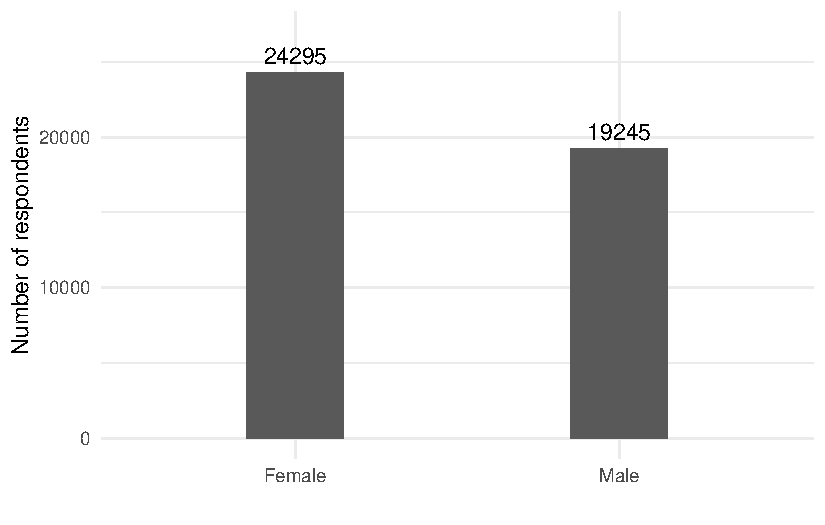
\includegraphics{paper_files/figure-pdf/fig-gender-histogram-1.pdf}

}

\caption{\label{fig-gender-histogram}Gender Distribution}

\end{figure}

The gender variable stores the responses of the respondent to a question
which asks them to choose between ``Male'' and ``Female'' as their only
two options to describe their gender. This question would have been
better phrased if it were asking for biological sex assigned at birth
rather than gender based on the options provided to the respondents.
Even though the survey asks for the respondent's sexual orientation
later, the phrasing of this question alone could be a reason for people
to not submit their survey responses as they don't identify with the
given options which may lead to under-representation of people belonging
to this demographic in the dataset.

In Figure~\ref{fig-gender-histogram}, we can see the number of
respondents who identified as male and female. According to {``The
Gender Ratio of United States of America (2020 - 2028, Males Per 100
Females)''} (2024), the United States had a gender ratio of 97.14 males
to 100 females in 2020. Our data consists of 24,295 females and 19,245
male - the gender ratio represented here is considerably below the
national average at the time of the survey - this might introduce some
bias into our data.

\hypertarget{sec-data-voted-for}{%
\subsection{Voted For (CC20\_410)}\label{sec-data-voted-for}}

\begin{figure}

{\centering 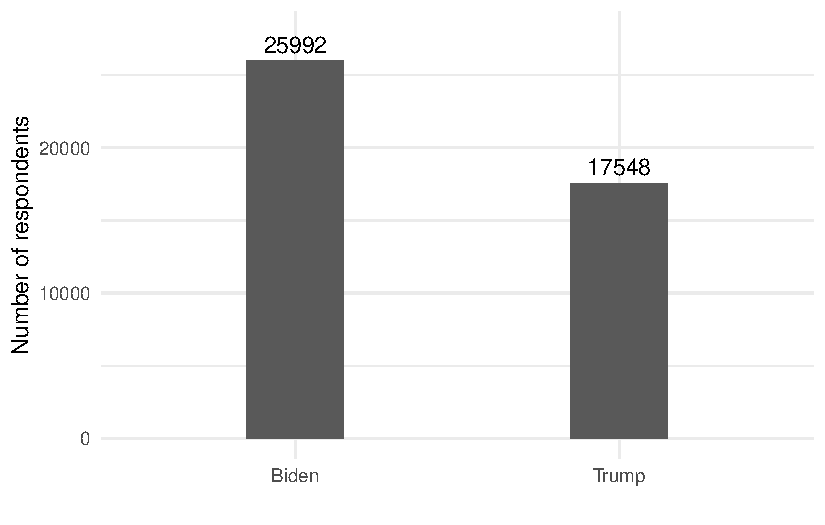
\includegraphics{paper_files/figure-pdf/fig-vote-histogram-1.pdf}

}

\caption{\label{fig-vote-histogram}Vote Distribution}

\end{figure}

The CC20\_410 variable, renamed to ``voted\_for'', records who the
respondent voted for in the 2020 Presidential Elections. The respondents
were given options other than Joe Biden and Donald Trump for this
question, such as ``Other'', ``I dd not vote'', ``Not Sure'', etc, but
these options were removed as they weren't needed for our purposes.

In Figure~\ref{fig-vote-histogram}, we can see that Biden has an
overwhelming majority over Trump in terms of popularity, with around a
6,000 vote difference between the two.

\hypertarget{sec-data-generation}{%
\subsection{Generation (and birthyear)}\label{sec-data-generation}}

\begin{figure}

{\centering 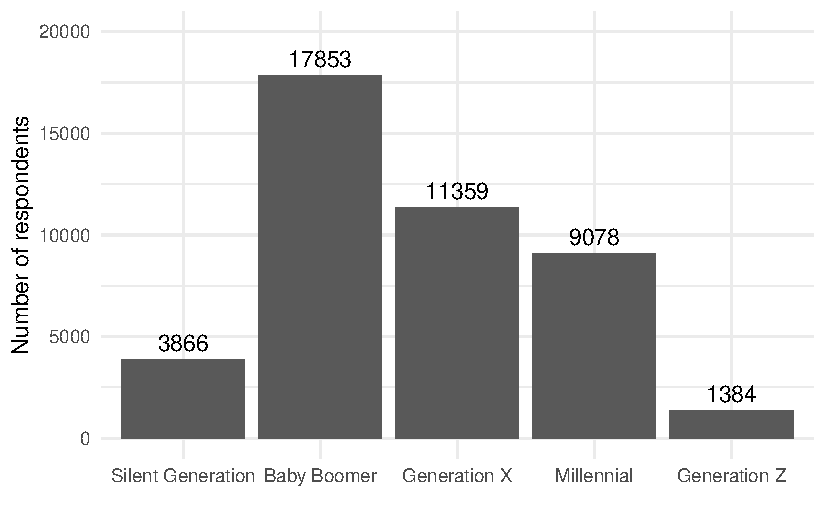
\includegraphics{paper_files/figure-pdf/fig-generation-histogram-1.pdf}

}

\caption{\label{fig-generation-histogram}Generation Distribution}

\end{figure}

The generation variable was created from the ``birthyr'' variable in the
dataset, where respondents recorded their year or birth. Each respondent
was assigned a ``generation'' according to their year of birth. The
generation breakpoints used for this paper are defined by Pew Research
Center (Dimock (2019)) as follows:

\begin{itemize}
\item
  Silent Generation: 1928 - 1945
\item
  Baby Boomer: 1946 - 1964
\item
  Generation X: 1965 - 1980
\item
  Millennial: 1981 - 1996
\item
  Generation Z: 1997 - 2012
\end{itemize}

Any respondents whose year of birth falls outside of these year ranges
were removed from the dataset. These numbers fall in line with the voter
turnout

In Figure~\ref{fig-generation-histogram}, we can see that Baby Boomers
show the largest representation of all groups. Generation X and
Millennial have similar number of respondents, and Silent Generation and
Generation Z have the lowest number of respondents. This distribution
falls in line with the voter turnout by age statistic reported by Pew
Research Center (Gramlich (2020)). Note that even though Generation Z
had the highest voter turnout for all generations (Dimock (2019)) and
their numbers look low compared to others, it falls in line with
expected numbers as the oldest Generation Z respondent who would've been
able to vote would've been born in 2002, leaving a considerable
population of this generation unable to vote.

\hypertarget{sec-model}{%
\section{Model}\label{sec-model}}

We will be using logistic regression to model our data, where our
outcome variable would be whether a respondent prefers Biden as the
presidential candidate. Gender and generation will be used as predictors
our outcome variable.

\hypertarget{model-set-up}{%
\subsection{Model set-up}\label{model-set-up}}

Define:

\begin{itemize}
\item
  \(y_i\) is the political preference of the respondent and equal to 1
  if Biden, and 0 if Trump
\item
  \(\mbox{gender}_i\) is the gender of the respondent
\item
  \(\mbox{generation}_i\) is the generation of the respondent
\end{itemize}

\begin{align} 
y_i|\pi_i &\sim \mbox{Bern}(\pi_i) \\
\mbox{logit}(\pi_i) &= \beta_0 + \beta_1 \times \mbox{gender}_i +  \beta_2 \times \mbox{generation}_i\\
\beta_0 &\sim \mbox{Normal}(0, 2.5) \\
\beta_1 &\sim \mbox{Normal}(0, 2.5) \\
\beta_2 &\sim \mbox{Normal}(0, 2.5)
\end{align}

We run the model in R (R Core Team 2023) using the \texttt{rstanarm}
package of Goodrich et al. (2022). We use the default priors from
\texttt{rstanarm}.

\hypertarget{model-justification}{%
\subsubsection{Model justification}\label{model-justification}}

Logistic regression is employed for this model since our variable of
interest can be constructed as a binary outcome variable - respondent
prefers Biden, respondent doesn't prefer Biden (prefers Trump). Logistic
regression is well suited for situations where the outcome variable
represents two mutually exclusive categories and its probability is
based on a set of predictor variables (here, gender and generation).

According to the common beliefs in our society as established in
Section~\ref{sec-intro}, we expect to see a positive relationship in the
younger generations, who we expect to be more left-leaning and therefore
be more favorable towards Biden. And vice versa, we expect to see a
negative relationship in the older generations, who we expect to be more
right leaning, and therefore, more conservative. However, due to the
large dissatisfaction in the majority of US citizens in 2020 due to how
President Trump handled the COVID pandemic (Jurkowitz (2020)), this skew
might not be as great as it could be for other elections. Regardless, we
expect to see a linear relationship between a person's generation and
preference for Biden - younger generational cohorts leaning more towards
voting for Biden.

The relationship between gender and political preference is a bit more
complicated. According to articles from the Conversation (Rosie Campbell
(2023)) and the Gallup (Saad (2024)), women tend to vote more
conservative than men before 2017, after which this trend flipped on its
head and women are began to vote more liberally.

\hypertarget{sec-results}{%
\section{Results}\label{sec-results}}

Our results are summarized in.

\begin{figure}

{\centering 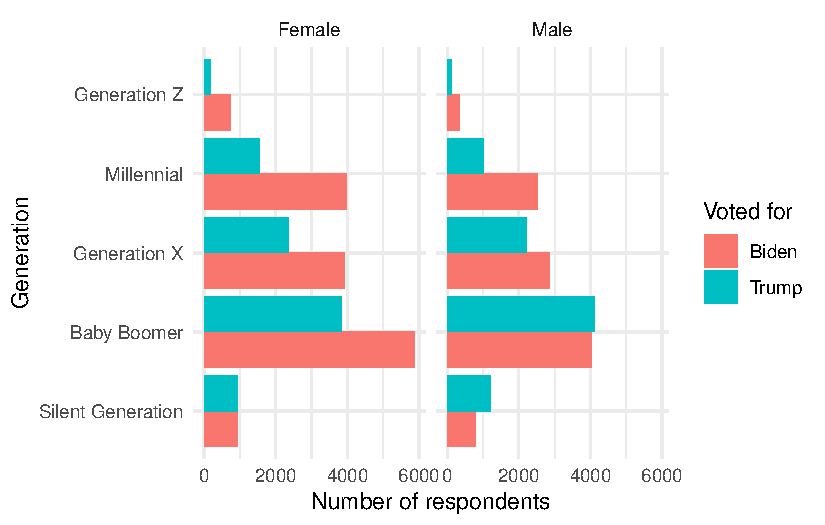
\includegraphics{paper_files/figure-pdf/fig-pres-pref-gender-generation-1.pdf}

}

\caption{\label{fig-pres-pref-gender-generation}Distribution of
presidential preferences, by gender, and by generation}

\end{figure}

Figure~\ref{fig-pres-pref-gender-generation} Compares the political
preferences between respondents of different generations, separated by
gender. The voting behaviour on this histogram closely resembles most of
our assumptions, but there are some interesting observations which
weren't predicted.

First big observation is the fact that as generational cohorts get
younger, the difference in votes cast to Biden and Trump increase in the
favor of Biden across both genders, showing that younger voters tend to
be more liberally aligned politically. This phenomenon is exaggerated in
the female voter base of each generation - the difference between the
votes cast to Biden and Trump are much greater compared to those in
males.

Between the two genders, female voters showed a much higher discrepancy
in their voting preferences in the favour of Biden. This falls in line
with the recent trends of women voting more liberal in the recent years.

Note that these observations are further supported by the coefficients
of our fitted logistic model, as seen in Figure~\ref{fig-model-summary}:

\begin{figure}

{\centering 

\hypertarget{fig-model-summary-1}{}
\begin{table}
\centering
\begin{tabular}[t]{lc}
\toprule
  & Support Biden\\
\midrule
(Intercept) & \num{0.051}\\
 & (\num{0.035})\\
generationBaby Boomer & \num{-0.422}\\
 & (\num{0.036})\\
generationGeneration X & \num{-0.597}\\
 & (\num{0.040})\\
generationMillennial & \num{-1.116}\\
 & (\num{0.041})\\
generationGeneration Z & \num{-1.393}\\
 & (\num{0.070})\\
genderMale & \num{0.328}\\
 & (\num{0.020})\\
\midrule
Num.Obs. & \num{43540}\\
R2 & \num{0.034}\\
Log.Lik. & \num{-28594.228}\\
ELPD & \num{-28600.2}\\
ELPD s.e. & \num{54.6}\\
LOOIC & \num{57200.4}\\
LOOIC s.e. & \num{109.3}\\
WAIC & \num{57200.3}\\
RMSE & \num{0.48}\\
\bottomrule
\end{tabular}
\end{table}

}

\caption{\label{fig-model-summary}Model Summary}

\end{figure}

Note that for our model, we set Biden as our reference level for
voted\_for, Silent Generation as our reference level for generation, and
Female as our reference level for gender. This means that the
coefficients of other generations are relative to the Silent Generation,
which we have seen from the histogram tend to favor Trump over Biden.
Moreover, R treats ``Biden'' as our failure case and ``Trump'' as our
success case, which implies that negative coefficients imply a positive
increase in odds for Biden. Conversely, a positive coefficient imply a
decrease in odds for voting Biden, i.e., an increase in odds of voting
for Trump. Keeping these key pieces of information in mind, we proceed
to our model's results.

Our model arrived at the intercept of 0.051 with a standard error of
0.035. This means that we can say with fairly high accuracy, that when
all predictors are set to 0, i.e, for the female demographic of the
Silent Generation, Trump's log odds for getting a vote is 0.051, which
is about 51\% probability - this falls in line with our observations in
Figure~\ref{fig-pres-pref-gender-generation}.

Keeping our reference level of Silent Generation and Biden in mind, we
now observe the coefficients for different generations:

\begin{itemize}
\item
  Baby Boomers have a coefficient of -0.422 with a standard error of
  0.036
\item
  Generation X has a coefficient of -0.597 with a standard error of
  0.040
\item
  Millennials have a coefficient of -1.116 with a standard error of
  0.041
\item
  Generation Z have a coefficient of -1.393 with a standard error of
  0.070
\end{itemize}

Notice that the coefficients tend to decrease further and further as the
generational cohorts become younger, implying that Biden tends to gain
more favor as the generational cohorts get younger - keeping in line
with our hypothesis. Moreover, the standard error for each of these
generations is very small, implying a high precision to these
predictions made by our model.

Finally, we observe the coefficient for male gender to be 0.328 with a
standard error of 0.020, which when compared to the female gender favors
Trump over Biden. This implies that male respondents showed an increase
of 0.328 log odds in voting for Trump when compared to female
respondents. And due to our very low standard error, we can say with
high confidence that male respondents have a higher chance of voting for
Trump compared to female respondents, which also agrees with our
hypothesis.

\hypertarget{sec-discussion}{%
\section{Discussion}\label{sec-discussion}}

\hypertarget{sec-first-point}{%
\subsection{What was done}\label{sec-first-point}}

It is an age old belief that as a person starts out with a left leaning
political compass and as they get older, their ideology slowly shifts
over to the right. The purpose of this paper was to test this belief by
gaining a better understanding of the voting preferences (between Joe
Biden and Donald J. Trump) different generations had in the 2020 US
Presidential Elections, based on the generation they belonged to, as
well as the gender of the members of these generations. This was done by
obtaining data from the 2020 CES Common Consent dataset, which contained
survey responses from over 61,000 adults surveyed over the internet.
Initial exploratory data analysis suggested that younger generations
tended to favor Biden over Trump, and women tended to favor Biden more
heavily than men of the same generation. Logistic regression modelling
was then used to formalize this discovery, and it showed a clear trend
which agreed with our initial hypothesis - as generational cohorts get
younger, the odds of favoring Biden increase.

\hypertarget{younger-generations-vote-liberally-older-generations-vote-conservative}{%
\subsection{``Younger Generations vote Liberally; Older Generations vote
Conservative''}\label{younger-generations-vote-liberally-older-generations-vote-conservative}}

Our main hypothesis of the study was proven to be true from our findings
- younger generations vote liberally; older generations vote
conservative. From both exploratory analysis and our model, it was found
that younger generations, such as Millennial and Generation Z, tend to
favor supporting liberal candidates (Biden in this case). As
generational cohorts got older, their liberal support slowly decreased
until eventually the generation as a whole tended to favor the
conservative candidate (Trump). Do note that even though Trump's
favorability increased as generations got older, Biden still held
majority votes across all generations other than the Silent Generation,
who are now a minority in the American voter base. This might be
explained by Trump's growing unpopularity in 2020 from the way he
handled the COVID-19 pandemic, and over his term as the President as a
whole. What's more interesting is that even though only a part of
Generation Z participated in the election, and it was the first election
for the generation as a whole, they fit in the trend perfectly, showing
overwhelming support for Biden in their votes compared to other
generations, even more so than Millennials.

\hypertarget{women-vote-more-liberally-than-men}{%
\subsection{``Women Vote more Liberally than
Men''}\label{women-vote-more-liberally-than-men}}

A number of studies published in the last few years (Saad (2024), Rosie
Campbell (2023)) suggested that women were voting more liberally than
before, and this was observed in our own findings as well. Against the
traditional beliefs that women tended to vote more conservative than
men, it was found that women were tended to favor the liberal candidate
much greater than the conservative candidates across all generations.

\hypertarget{weaknesses-and-next-steps}{%
\subsection{Weaknesses and next steps}\label{weaknesses-and-next-steps}}

Some weaknesses of this model arrive from the data that was used for
this study - the 2020 CES Common Consent dataset. Even though it had
over 61,000 respondents, over 6,000 respondents either didn't register
to vote or had no idea if they were registered at all. Moreover, after
data cleaning was completed, we were left with 43,540 entries in the
dataset - over a third of the data was lost. Furthermore, in these
43,540 entries, the ratio of male to female entries weighed greatly in
favor of females, and was much higher than the national gender ratio in
2020.

Due to the nature of the survey being online, a significant portion of
the US's demographics was left out of the pool. It is estimated that in
2020 about 13\% of the US population did not have access to the internet
(Petrosyan (2024)), which leads to the exclusion of about 43 million
citizens being excluded from the survey with no representation at all.

It would be interesting to study how different generations tend to vote
in the previous US presidential elections (which occurred under more
normal circumstances) as well, especially the cases where a new
generation was added to the voter pool of the nation, similar to 2020.
Another interesting avenue would be to study voting trends amongst women
over the last few decades, as the scope of this paper limits us from
exploring exactly how great of a shift occurred in 2017.

\newpage

\appendix

\hypertarget{appendix}{%
\section*{Appendix}\label{appendix}}
\addcontentsline{toc}{section}{Appendix}

\hypertarget{sec-model-details}{%
\section{Model details}\label{sec-model-details}}

\hypertarget{posterior-predictive-check}{%
\subsection{Posterior predictive
check}\label{posterior-predictive-check}}

In Figure~\ref{fig-ppcheckandposteriorvsprior-1} we implement a
posterior predictive check. In
Figure~\ref{fig-ppcheckandposteriorvsprior-2} we compare the posterior
with the prior.

\begin{figure}

\begin{minipage}[t]{0.50\linewidth}

{\centering 

\raisebox{-\height}{

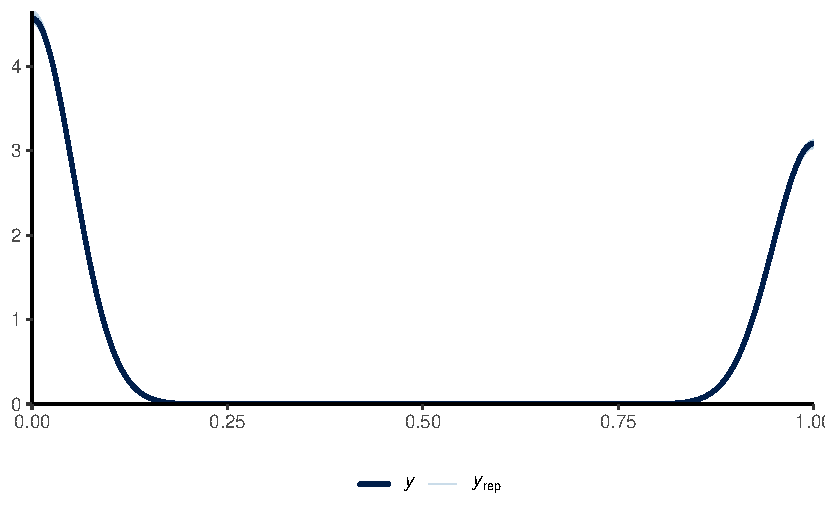
\includegraphics{paper_files/figure-pdf/fig-ppcheckandposteriorvsprior-1.pdf}

}

}

\subcaption{\label{fig-ppcheckandposteriorvsprior-1}Posterior prediction
check}
\end{minipage}%
%
\begin{minipage}[t]{0.50\linewidth}

{\centering 

\raisebox{-\height}{

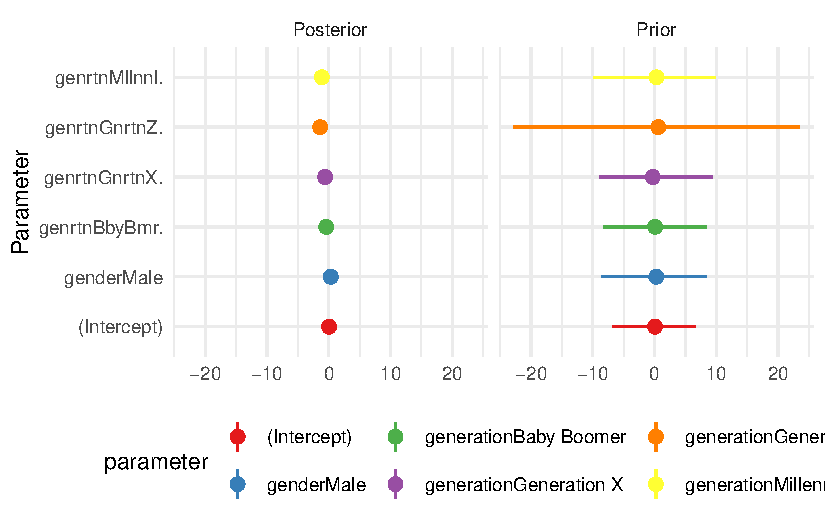
\includegraphics{paper_files/figure-pdf/fig-ppcheckandposteriorvsprior-2.pdf}

}

}

\subcaption{\label{fig-ppcheckandposteriorvsprior-2}Comparing the
posterior with the prior}
\end{minipage}%

\caption{\label{fig-ppcheckandposteriorvsprior}Examining how the model
fits, and is affected by, the data}

\end{figure}

\hypertarget{diagnostics}{%
\subsection{Diagnostics}\label{diagnostics}}

\begin{figure}

{\centering 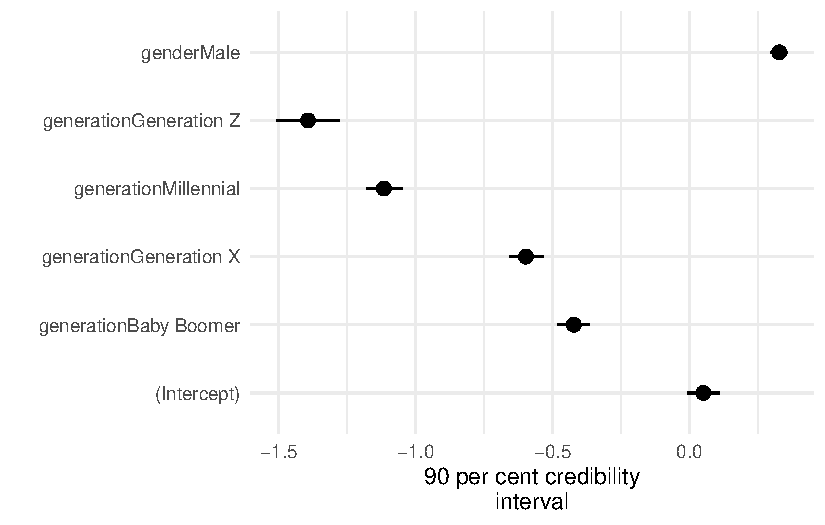
\includegraphics{paper_files/figure-pdf/fig-model-cred-interval-1.pdf}

}

\caption{\label{fig-model-cred-interval}Credible Intervals}

\end{figure}

\begin{figure}

\begin{minipage}[t]{0.50\linewidth}

{\centering 

\raisebox{-\height}{

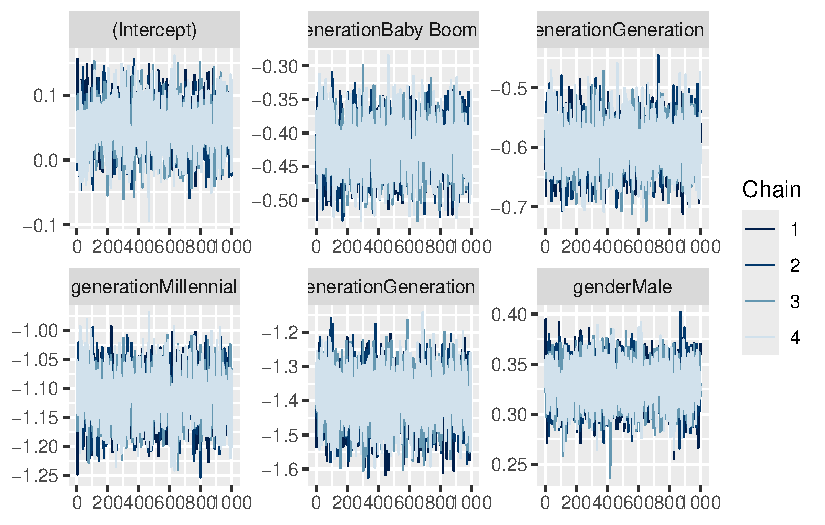
\includegraphics{paper_files/figure-pdf/fig-model-trace-rhat-1.pdf}

}

\caption{\label{fig-model-trace-rhat-1}Trace plot}

}

\end{minipage}%
%
\begin{minipage}[t]{0.50\linewidth}

{\centering 

\raisebox{-\height}{

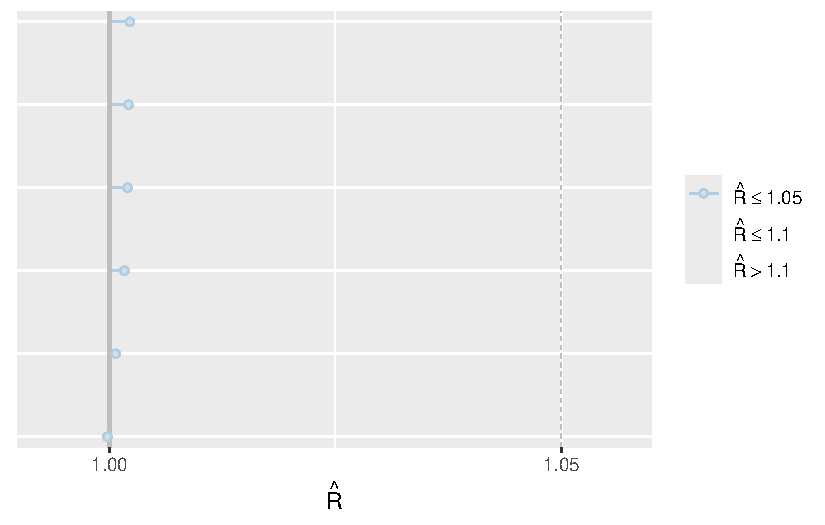
\includegraphics{paper_files/figure-pdf/fig-model-trace-rhat-2.pdf}

}

\caption{\label{fig-model-trace-rhat-2}Rhat plot}

}

\end{minipage}%

\end{figure}

\newpage

\hypertarget{references}{%
\section*{References}\label{references}}
\addcontentsline{toc}{section}{References}

\hypertarget{refs}{}
\begin{CSLReferences}{1}{0}
\leavevmode\vadjust pre{\hypertarget{ref-2020voterturnout}{}}%
\emph{2020 Presidential Election Voting and Registration Tables Now
Available}. 2021. United States Census Bureau.
\url{https://www.census.gov/newsroom/press-releases/2021/2020-presidential-election-voting-and-registration-tables-now-available.html}.

\leavevmode\vadjust pre{\hypertarget{ref-citeModelsummary}{}}%
Arel-Bundock, Vincent. 2022. {``{modelsummary}: Data and Model Summaries
in {R}.''} \emph{Journal of Statistical Software} 103 (1): 1--23.
\url{https://doi.org/10.18637/jss.v103.i01}.

\leavevmode\vadjust pre{\hypertarget{ref-pewgenerations}{}}%
Dimock, Michael. 2019. {``Defining Generations: Where Millennials End
and Generation z Begins.''}
\url{https://www.pewresearch.org/short-reads/2019/01/17/where-millennials-end-and-generation-z-begins/}.

\leavevmode\vadjust pre{\hypertarget{ref-rstanarm}{}}%
Goodrich, Ben, Jonah Gabry, Imad Ali, and Sam Brilleman. 2022.
{``Rstanarm: {Bayesian} Applied Regression Modeling via {Stan}.''}
\url{https://mc-stan.org/rstanarm/}.

\leavevmode\vadjust pre{\hypertarget{ref-citeRstanarm}{}}%
---------. 2024. {``Rstanarm: {Bayesian} Applied Regression Modeling via
{Stan}.''} \url{https://mc-stan.org/rstanarm/}.

\leavevmode\vadjust pre{\hypertarget{ref-pewvoterturnout}{}}%
Gramlich, John. 2020. {``What the 2020 Electorate Looks Like by Party,
Race and Ethnicity, Age, Education and Religion.''}
\url{https://www.pewresearch.org/short-reads/2020/10/26/what-the-2020-electorate-looks-like-by-party-race-and-ethnicity-age-education-and-religion/}.

\leavevmode\vadjust pre{\hypertarget{ref-genzturnout}{}}%
Hess, Abigail Johnson. 2020. {``The 2020 Election Shows Gen z's Voting
Power for Years to Come.''}
\url{https://www.cnbc.com/2020/11/18/the-2020-election-shows-gen-zs-voting-power-for-years-to-come.html}.

\leavevmode\vadjust pre{\hypertarget{ref-washingtonpost}{}}%
Itkowitz, Colby. 2019. {``The Next Generation of Voters Is More Liberal,
More Inclusive and Believes in Government.''}
\url{https://www.washingtonpost.com/politics/2019/01/17/next-generation-voters-are-more-liberal-more-inclusive-believe-government/}.

\leavevmode\vadjust pre{\hypertarget{ref-trumpdisapproval}{}}%
Jurkowitz, Mark. 2020. {``Majority of Americans Disapprove of Trump's
COVID-19 Messaging, Though Large Partisan Gaps Persist.''}
\url{https://www.pewresearch.org/short-reads/2020/09/15/majority-of-americans-disapprove-of-trumps-covid-19-messaging-though-large-partisan-gaps-persist/\#:~:text=The\%20survey\%20also\%20finds\%20large,say\%20it\%20is\%20completely\%20wrong.}

\leavevmode\vadjust pre{\hypertarget{ref-dataverse}{}}%
Kuriwaki, Shiro, Will Beasley, and Thomas J. Leeper. 2023.
\emph{Dataverse: R Client for Dataverse 4+ Repositories}.

\leavevmode\vadjust pre{\hypertarget{ref-statista}{}}%
Petrosyan, Ani. 2024. {``United States Internet Penetration
2000-2024.''}
\url{https://www.statista.com/statistics/209117/us-internet-penetration/}.

\leavevmode\vadjust pre{\hypertarget{ref-citeR}{}}%
R Core Team. 2023. \emph{R: A Language and Environment for Statistical
Computing}. Vienna, Austria: R Foundation for Statistical Computing.
\url{https://www.R-project.org/}.

\leavevmode\vadjust pre{\hypertarget{ref-citeArrow}{}}%
Richardson, Neal, Ian Cook, Nic Crane, Dewey Dunnington, Romain
François, Jonathan Keane, Dragoș Moldovan-Grünfeld, Jeroen Ooms, Jacob
Wujciak-Jens, and Apache Arrow. 2024. \emph{Arrow: Integration to
'Apache' 'Arrow'}. \url{https://CRAN.R-project.org/package=arrow}.

\leavevmode\vadjust pre{\hypertarget{ref-conversationwomen}{}}%
Rosie Campbell, Rosalind Shorrocks. 2023. {``Women Used to Be More
Likely to Vote Conservative Than Men but That All Changed in 2017 -- We
Wanted to Find Out Why.''}
\url{https://theconversation.com/women-used-to-be-more-likely-to-vote-conservative-than-men-but-that-all-changed-in-2017-we-wanted-to-find-out-why-214019}.

\leavevmode\vadjust pre{\hypertarget{ref-gallupwomen}{}}%
Saad, Lydia. 2024. {``U.s. Women Have Become More Liberal; Men Mostly
Stable.''}
\url{https://news.gallup.com/poll/609914/women-become-liberal-men-mostly-stable.aspx}.

\leavevmode\vadjust pre{\hypertarget{ref-datasheet}{}}%
Schaffner, Brian, Stephen Ansolabehere, and Sam Luks. 2021b.
{``{Cooperative Election Study Common Content, 2020}.''} Harvard
Dataverse. \url{https://doi.org/10.7910/DVN/E9N6PH}.

\leavevmode\vadjust pre{\hypertarget{ref-dataset}{}}%
---------. 2021a. {``{Cooperative Election Study Common Content,
2020}.''} Harvard Dataverse. \url{https://doi.org/10.7910/DVN/E9N6PH}.

\leavevmode\vadjust pre{\hypertarget{ref-genderratio}{}}%
{``The Gender Ratio of United States of America (2020 - 2028, Males Per
100 Females).''} 2024. GlobalData.
\url{https://www.globaldata.com/data-insights/macroeconomic/the-gender-ratio-of-united-states-of-america-325511/}.

\leavevmode\vadjust pre{\hypertarget{ref-citeGgplot2}{}}%
Wickham, Hadley. 2016. \emph{Ggplot2: Elegant Graphics for Data
Analysis}. Springer-Verlag New York.
\url{https://ggplot2.tidyverse.org}.

\leavevmode\vadjust pre{\hypertarget{ref-tidyverse}{}}%
Wickham, Hadley, Mara Averick, Jennifer Bryan, Winston Chang, Lucy
D'Agostino McGowan, Romain François, Garrett Grolemund, et al. 2019.
{``Welcome to the {tidyverse}.''} \emph{Journal of Open Source Software}
4 (43): 1686. \url{https://doi.org/10.21105/joss.01686}.

\leavevmode\vadjust pre{\hypertarget{ref-citeDplyr}{}}%
Wickham, Hadley, Romain François, Lionel Henry, Kirill Müller, and Davis
Vaughan. 2023. \emph{Dplyr: A Grammar of Data Manipulation}.
\url{https://CRAN.R-project.org/package=dplyr}.

\leavevmode\vadjust pre{\hypertarget{ref-citeTidyr}{}}%
Wickham, Hadley, Davis Vaughan, and Maximilian Girlich. 2023.
\emph{Tidyr: Tidy Messy Data}.
\url{https://CRAN.R-project.org/package=tidyr}.

\leavevmode\vadjust pre{\hypertarget{ref-citeKnitr}{}}%
Xie, Yihui. 2015. \emph{Dynamic Documents with {R} and Knitr}. 2nd ed.
Boca Raton, Florida: Chapman; Hall/CRC. \url{https://yihui.org/knitr/}.

\end{CSLReferences}



\end{document}
